\documentclass{article}
\usepackage{listings}
\usepackage{amsmath}
\usepackage{subfig}
\usepackage{amsthm}
\usepackage{amssymb}
\usepackage{fullpage}
\usepackage{graphicx}
\usepackage{mdwlist}
\usepackage{geometry}
\usepackage{titlesec}
\usepackage{palatino}
\usepackage{mathrsfs}
\usepackage{fancyhdr}
\usepackage{fancyvrb}
\usepackage{paralist}
\usepackage{todonotes}
\usepackage{tikz}
\usepackage{float} % Place figures where you ACTUALLY want it
\usepackage{comment} % A hack to toggle sections
\usepackage{ifthen}
\usepackage{mdframed}
\usepackage{verbatim}
\usepackage{listings}
\usepackage{booktabs}
\usepackage{bbm}
\usepackage{upquote} % Prevents backticks replacing single-quotes in verbatim
\usepackage[strings]{underscore}
\usepackage[colorlinks=true]{hyperref}
\usetikzlibrary{positioning,shapes,backgrounds}

\usepackage{algorithm}
\usepackage[noend]{algpseudocode}
\algnewcommand{\LeftComment}[1]{\Statex \(\triangleright\) #1}

\geometry{margin=1in}
\geometry{headheight=2in}
\geometry{top=2in}

\setlength{\marginparwidth}{2.15cm}
\setlength{\parindent}{0em}
\setlength{\parskip}{0.6\baselineskip}

\rhead{}
\lhead{}

% Spacing settings.
\titlespacing\section{0pt}{12pt plus 2pt minus 2pt}{0pt plus 2pt minus 2pt}
\titlespacing\subsection{0pt}{12pt plus 4pt minus 2pt}{0pt plus 2pt minus 2pt}
\titlespacing\subsubsection{0pt}{12pt plus 4pt minus 2pt}{0pt plus 2pt minus 2pt}
\renewcommand{\baselinestretch}{1.15}

% Shortcuts for commonly used operators.
\newcommand{\E}{\mathbb{E}}
\newcommand{\Var}{\operatorname{Var}}
\newcommand{\Cov}{\operatorname{Cov}}
\newcommand{\Bias}{\operatorname{Bias}}
\DeclareMathOperator{\argmin}{arg\,min}
\DeclareMathOperator{\argmax}{arg\,max}

% Do not number subsections and below.
\setcounter{secnumdepth}{1}

% Custom format subsection.
\titleformat*{\subsection}{\large\bfseries}

% Set up the problem environment.
\newcounter{problem}[section]
\newenvironment{problem}[1][]
  {\begingroup
    \setlength{\parskip}{0em}
    \refstepcounter{problem}\par\addvspace{1em}\textbf{Problem~\Alph{problem}\!
    \ifthenelse{\equal{#1}{}}{}{ [#1 points]}:}
  \endgroup}

% Set up the subproblem environment.
\newcounter{subproblem}[problem]
\newenvironment{subproblem}[1][]
  {\begingroup
    \setlength{\parskip}{0em}
    \refstepcounter{subproblem}\par\medskip\textbf{\roman{subproblem}.\!
    \ifthenelse{\equal{#1}{}}{}{ [#1 points]:}}
  \endgroup}

% Set up the teachers and materials commands.
\newcommand\teachers[1]
  {\begingroup
    \setlength{\parskip}{0em}
    \vspace{0.3em} \textit{\hspace*{2em} TAs responsible: #1} \par
  \endgroup}
\newcommand\materials[1]
  {\begingroup
    \setlength{\parskip}{0em}
    \textit{\hspace*{2em} Relevant materials: #1} \par \vspace{1em}
  \endgroup}

% Set up the hint environment.
\newenvironment{hint}[1][]
  {\begin{em}\textbf{Hint: }}
  {\end{em}}


% Set up the solution environment.
\ifshowsolutions
  \newenvironment{solution}[1][]
    {\par\medskip \begin{mdframed}\textbf{Solution~\Alph{problem}#1:} \begin{em}}
    {\end{em}\medskip\end{mdframed}\medskip}
  \newenvironment{subsolution}[1][]
    {\par\medskip \begin{mdframed}\textbf{Solution~\Alph{problem}#1.\roman{subproblem}:} \begin{em}}
    {\end{em}\medskip\end{mdframed}\medskip}
\else
  \excludecomment{solution}
  \excludecomment{subsolution}
\fi

% Other commands and stuff
\newcommand{\RR}{\mathbb{R}} % typing \RR prints Blackboard R 
\newcommand{\NN}{\mathbb{N}} % typing \NN prints Blackboard N 
\newcommand{\ZZ}{\mathbb{Z}} % typing \ZZ prints Blackboard Z 

\newtheorem{theorem}{Theorem}[section]
\newtheorem{corollary}{Corollary}[theorem]
\newtheorem{lemma}[theorem]{Lemma}

\newcommand{\Lra}{\Leftrightarrow}
\newcommand{\lra}{\leftrightarrow}
\newcommand{\Ra}{\Rightarrow}
\newcommand{\ra}{\rightarrow}
\newcommand{\norm}[1]{\left\lVert#1\right\rVert}
\newcommand{\e}{\epsilon}



\title{Report for hw3 cs148}
\author{Akshay Yeluri}

\begin{document}
\maketitle{}

\subsection{Code inclusion}
You can see the code at my github repo @
https://github.com/akshayyeluri/caltech-ee148-spring2020-hw03.
In the repo, I'm also including the 2 jupyter notebooks I used
for developing my code. The first (model_building.ipynb) 
shows the process of developing the best CNN I could. The second
(analysis.ipynb) which is also attached to this report as a pdf, is the code
and the plots for questions 7 and 8 in the spec for this assignment.
The rest of the code that matters is of course in main.py.
The repo also has the models directory, which includes pytorch dumps
of the best model (best_model.pt), the original model trained without any
data augmentation (no_transform_model.pt), the original model with 
data augmentation (transform_V0.pt), and the models trained on subsets of training
data (model_sixteenth.pt, model_eighth.pt, etc). There's finally a plots
directory, including all the plots generated by analysis.ipynb.

\subsection{Results with and without augmentation}
I tried a few different transforms including cropping and normalizing. The
cropping didn't really seem to help, but the normalization did make the original
model perform better. I just normalized using 
`transforms.Normalize((0.1307,), (0.3081,))', which uses the mean and std
of the train set.

\par
Results without data augmentation (no_transform_model.pt):
Train loss=0.1690, accuracy=97.3,
Test loss=0.1614, accuracy=97.4

\par
Results with data augmentation (transform_V0.pt):
Train loss=0.0813, accuracy=97.6, 
Test loss=0.0774, accuracy=97.5

\par
What you can see is that the train and test loss both are lower with the
normalization. Also the accuracy gets better as well.

\subsection{Developing best CNN}
The process I went through to develop my architecture was essentially just a lot
of trial and error. I followed some guiding principles, like not condensing too
much in one layer, and making sure to only reduce the image size slightly in
each layer. I also tried to make sure that there was a nonlinearity and a
maxpool between each conv layer, because when I removed the maxpool layers the
performance got a lot worse. I also literally exhaustive searched to find the
probability in my dropout layer.
One trick I used a lot was testing different model's performances after one
epoch, as a proxy for how good the models would be after training. But anyway,
after a while I converged on the final model, which seems to work well.
I'm including the learning curves (the train and test loss) for the original
model without transforms, the original model with transforms, and the final
model

\begin{figure}[H]
\caption{Learning curves for original model with no transforms / data augmentation}
\centering
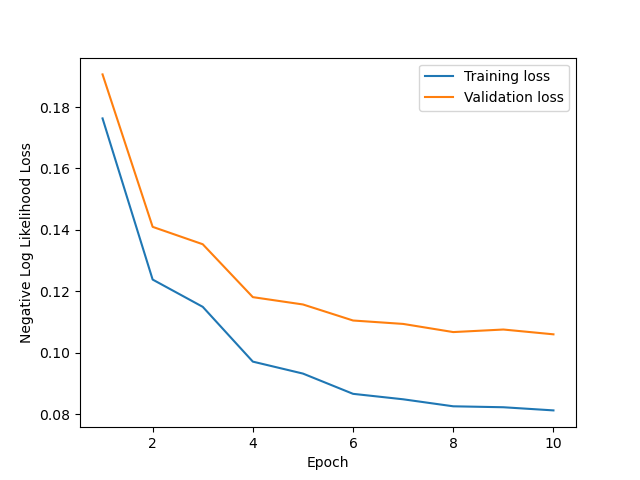
\includegraphics[width=0.6\textwidth]{plots/no_transform_curves.png}
\end{figure}

\begin{figure}[H]
\caption{Learning curves for original model with transforms / data augmentation}
\centering
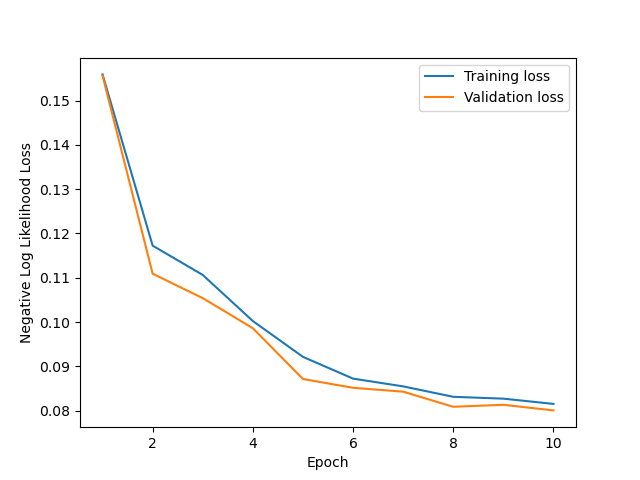
\includegraphics[width=0.6\textwidth]{plots/transform_V0_curves.png}
\end{figure}

\begin{figure}[H]
\caption{Learning curves for final model}
\centering
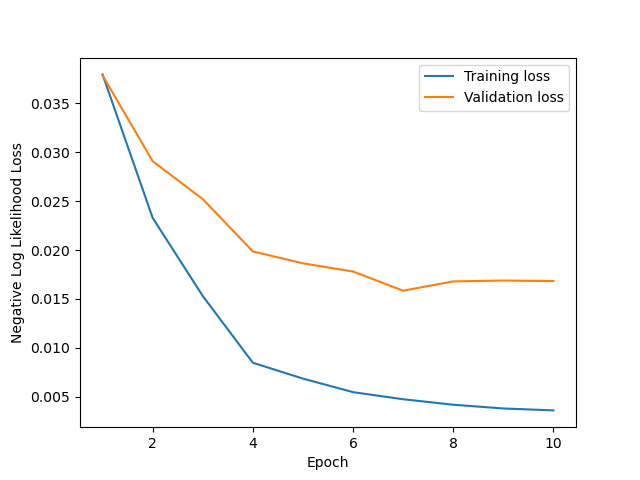
\includegraphics[width=0.6\textwidth]{plots/best_model_curves.png}
\end{figure}

\subsection{Rest of the analysis}
The rest of the analysis is attached as a separate pdf generated from
analysis.ipynb.

\end{document}

